\chapter{Support Vector Machine }
\label{chapter:SVM}
\section{SVM(Support Vector Machine)介紹}
SVM是一種線性分類器,可以處理線性分類問題如圖\ref{fig:Linear},同時卻也可以推展到解決非線性如圖\ref{fig:unkinear}的分割問題。將在低維度空間線性不可分的樣本映射到高維度空間去使 SVM 能在高維空間當中建構超平面如圖\ref{fig:overspace}或超平面集合,進而將原始數據進行分類,找到一個超平面將這些樣本做有效的切割,而這個超平面兩邊的樣本要盡可能地遠離這個超平面,為了將來多出新的資料時也能有效,而為了能針對不同類型的數據有個別的分類效果,
通常會選擇適當的核函式(kernel function)來使用,SVM 的主要如下公式:
\begin{equation}
	\label{equ:SVM}
	_{w,\delta_i}^{min}\frac{1}{2}W^TW+C\sum_{i=1}^{n}\delta_i
\end{equation}
其中 w 為超平面的法向量,$\delta_i$超平面的容忍邊界參數,值越大容忍範圍越大,
C 為調整容忍邊界參數的權重。




\begin{figure}[h]
	\centerline{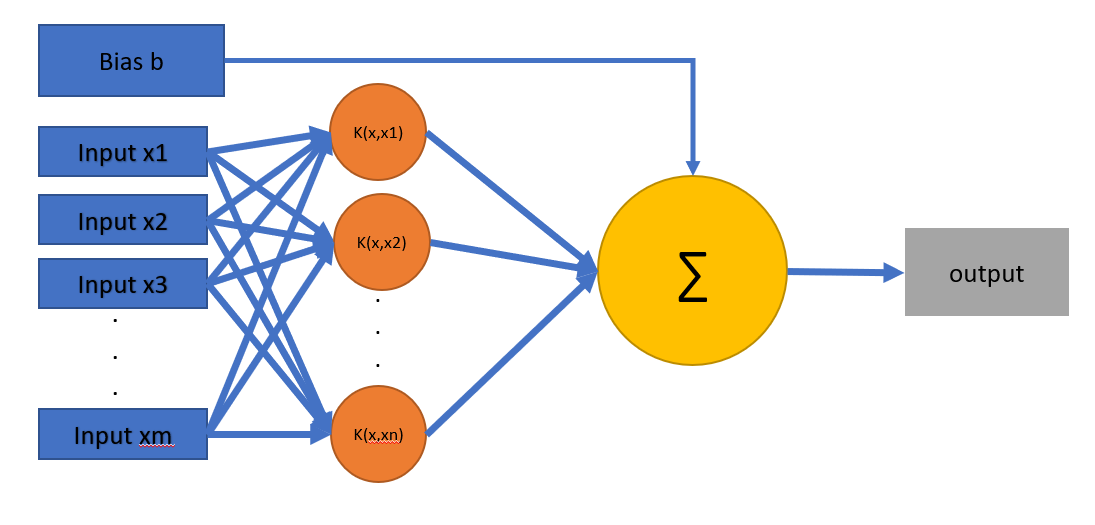
\includegraphics[height=8cm]{pic/SVM ar.PNG}}
	\caption{svm架構圖}
	\label{fig:svmar}
\end{figure}
\begin{figure}[h]
	\centerline{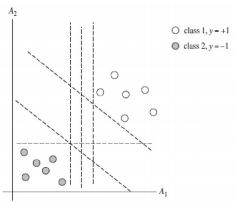
\includegraphics[height=8cm]{pic/SVML.png}}
	\caption{svm示意圖}
	\label{fig:svmar}
\end{figure}
\begin{figure}[H]
	\centerline{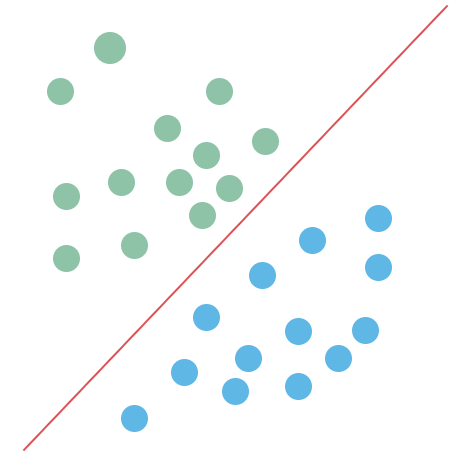
\includegraphics[height=5cm]{pic/linear.PNG}}
	\caption{線性可分示意圖}
	\label{fig:Linear}
\end{figure}
\begin{figure}[H]
	\centerline{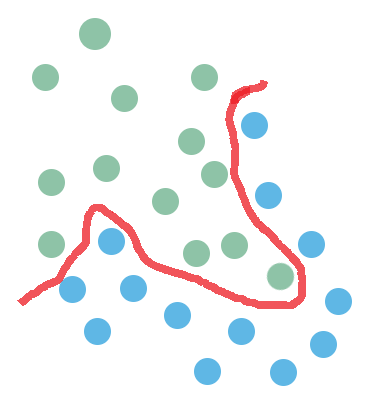
\includegraphics[height=5cm]{pic/unlinear.PNG}}
	\caption{線性不可分示意圖}
	\label{fig:unkinear}
\end{figure}

\begin{figure}[H]
	\centerline{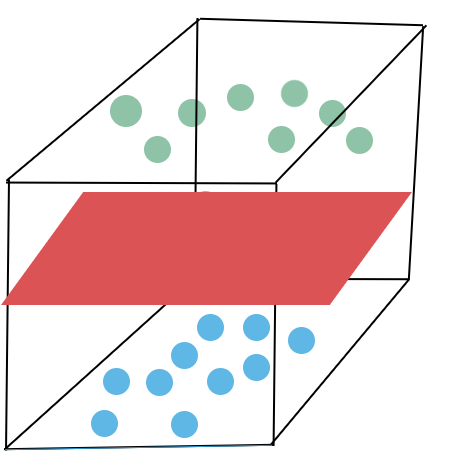
\includegraphics[height=5cm]{pic/over space.PNG}}
	\caption{超空間示意圖}
	\label{fig:overspace}
\end{figure}
\label{sec:background}

\section{核函數(kernel function)}
\begin{enumerate}
	\item
	      Linear Kernel
	      \begin{equation}
		      \label{Linear Kerne}
		      K(x,x')=x^Tx'
	      \end{equation}

	\item
	      Radial Basis Function Kernel
	      \begin{table}[h!]
		      \centering
		      \label{tab:rbf_table}
		      \begin{tabular}{ccc}
\toprule
  & RBF的名字 & 方程式 (\(r = ||\mathbf{C-X_i}||\) )   \\ 
\midrule
  & Gaussian Function  & \(h(r) = e^{-\varepsilon r}\)      \\ \\ 
  & Linear radial Function  & \(h(r) = r\)      \\ \\
  & Multiquadric   & \(h(r) = \sqrt{1+(\varepsilon r)^2}\)       \\ \\
  & Inverse quadric  &  \(h(r) = \frac{1}{1+(\varepsilon r)^2}\)     \\ \\ 
  & Inverse Multiquadric  &  \(h(r) = \frac{1}{\sqrt{1+(\varepsilon r)^2}}\)     \\
\bottomrule
\end{tabular}

		      \caption{常見的Radial Basis Function}
	      \end{table}
	\item
	      Sigmoid Kernel
	      \begin{equation}
		      \label{Sigmoid Kerne}
		      S(t)=\frac{1}{1+e^{-t}}
	      \end{equation}


\end{enumerate}

\begin{figure}[H]
	\centerline{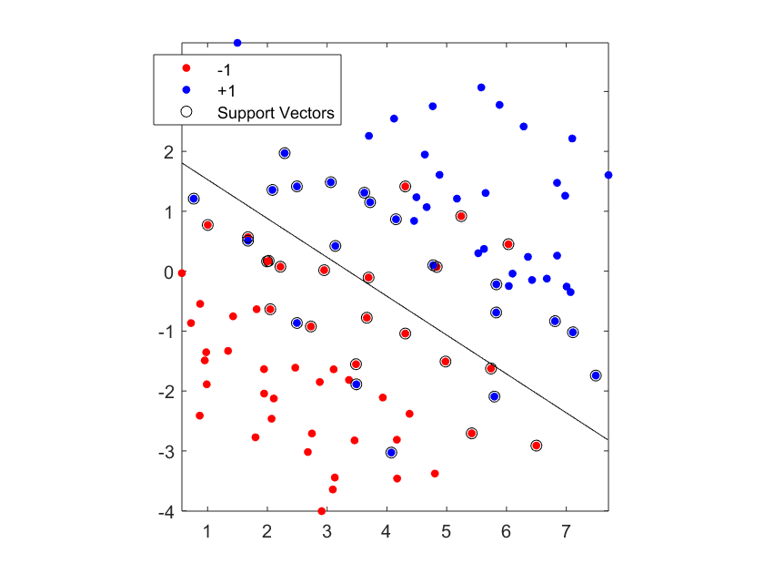
\includegraphics[height=5cm]{pic/linear kernel.png}}
	\caption{linear kernel示意圖}
	\label{fig:linear kernel}

	\centerline{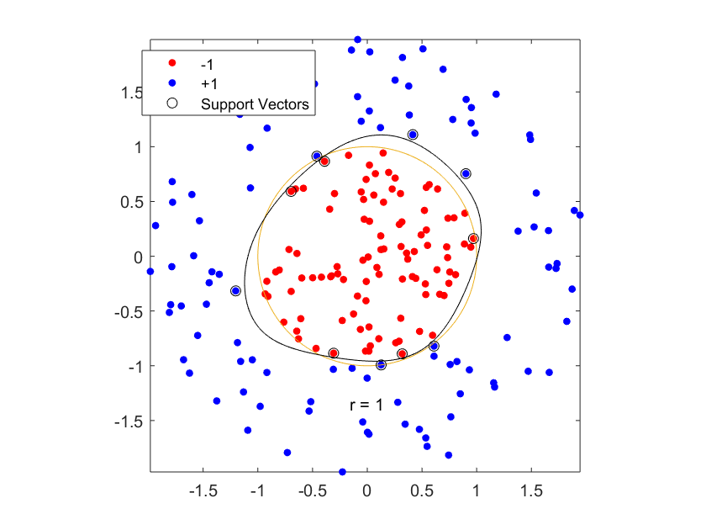
\includegraphics[height=5cm]{pic/Radial Basis Function Kernel.png}}
	\caption{Radial Basis Function Kernel示意圖}
	\label{fig:Radial Basis}

	\centerline{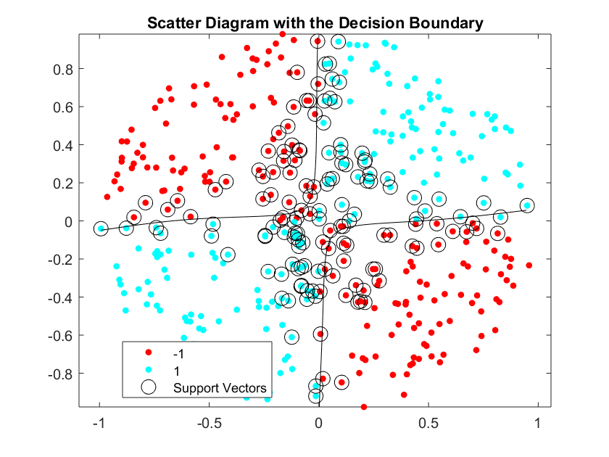
\includegraphics[height=5cm]{pic/Sigmoid Kernel.png}}
	\caption{Sigmoid Kernel示意圖}
	\label{Sigmoid Kernel}
\end{figure}
